\documentclass[tikz,border=5mm,12pt]{standalone}
\usepackage[fontsize=16pt]{fontsize}
\usepackage{drawutil}
\usetikzlibrary{arrows.meta}
\usetikzlibrary{positioning}

\def\xsep{15mm}
\begin{document}
  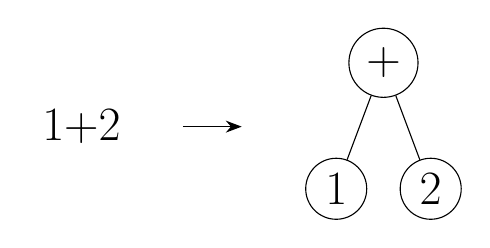
\begin{tikzpicture}[
    circled/.style={
      circle,draw,inner sep=3pt
    },
    arrowtip/.style={
      -{Stealth[scale=1.2]}
    },
    level distance=16mm,
    sibling distance=12mm
  ]
    \def\topText{\small\texttt{top}};

    \node (TokensA) at (0*\xsep,0) { \myfbox{1}\myfbox{+}\myfbox{2} };

    \node[right=27mm of TokensA,circled,yshift=6mm+6pt] (NodeBTop) { + }
      child { node[circled] { 1 } }
      child { node[circled] { 2 } };
    \coordinate[yshift=-6mm-6pt] (NodeB) at (NodeBTop);

    \draw[arrowtip,shorten <=6mm, shorten >=18mm] (TokensA) -- (NodeB);
  \end{tikzpicture}
\end{document}
